\chapter{原型系统设计与实现}

    原型系统包括核心工具Lapis和用户接口两大组件. 其中, 核心工具提供从脚本解析到测试生成与执行的整套方法的原型实现. 用户接口则包括核心工具的编程API接口, 在线API脚本的上传、编辑和可视化的web应用, 以及桌面端测试管理系统. 以上各部分完全独立.

	\section{核心工具Lapis}
	    \begin{figure}
	        \centering
	        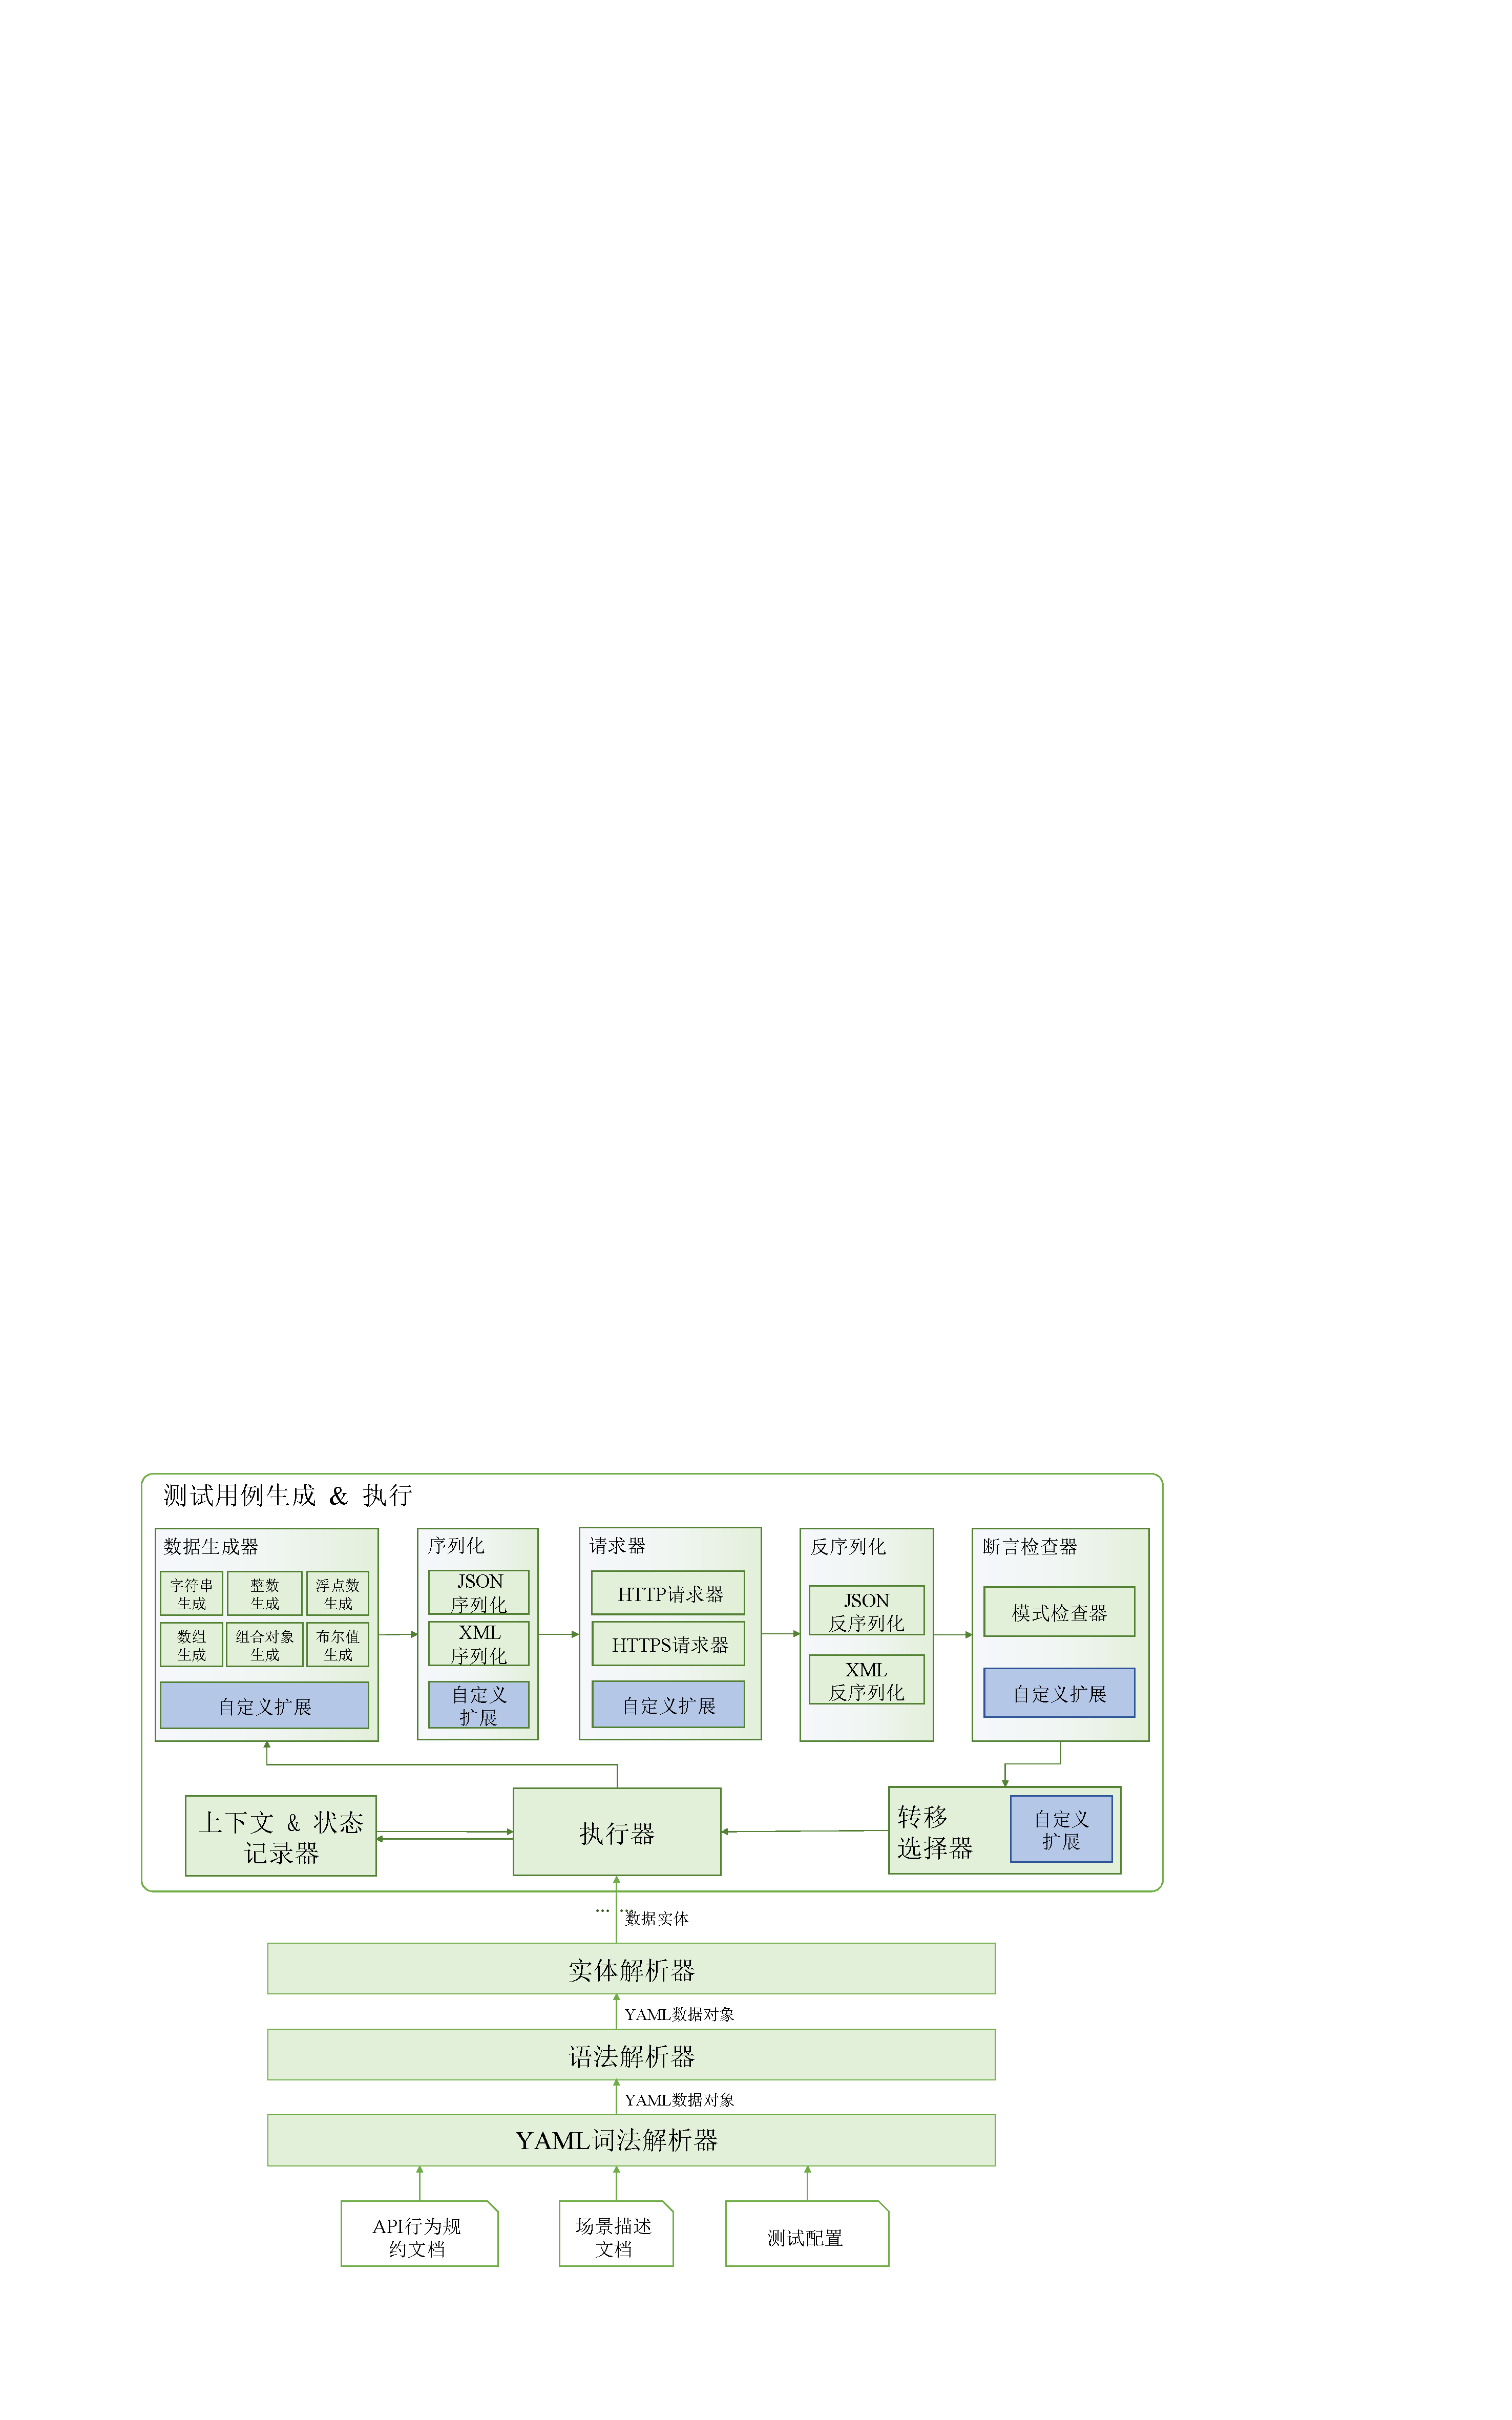
\includegraphics[width=300pt]{tool_architecture3.pdf}
	        \caption{Lapis工具整体结构.}
	        \label{fig:lapis_arch}
	    \end{figure}
	    
    	\subsection{脚本解析模块}
    
    	\subsection{测试生成模块}

	\section{用户接口}
		\subsection{编程接口}

		\subsection{web端脚本编辑系统}

		\subsection{*桌面端测试管理系统}


